
Representing the uncertain components of a query's output symbolically as a c-table makes a wide variety of integration techniques available for use in evaluating the statistical characteristics of the expression.  If our risk-management application assumes a general model of customer profit and customer satisfaction that relies on queries to create correlations between them, the sampler can detect this lack of dependency, estimate profit and probability of dissatisfaction separately, and combine the two afterwards.  Even with relatively straightforward integration techniques, additional knowledge of this form has a profoundly positive impact on the efficiency and accuracy with which expectations of query results can be computed.

Accuracy is especially relevant in cases where the integral has no closed form and exact methods are unavailable.  This is the case in a surprising range of practical applications, even when strong simplifying assumptions are made about the input data.  For example, even if the input data contains only independent variables sampled from well-studied distributions (e.g., the normal distribution), it is still possible for queries to create complex statistical dependencies in their own right.  It is well known, at least in the case of discrete and finite probability distributions, that relational algebra on block-independent-disjoint tables can construct any finite probability distribution\ \cite{1325861,IL1984}.

\begin{figure}
\begin{center}
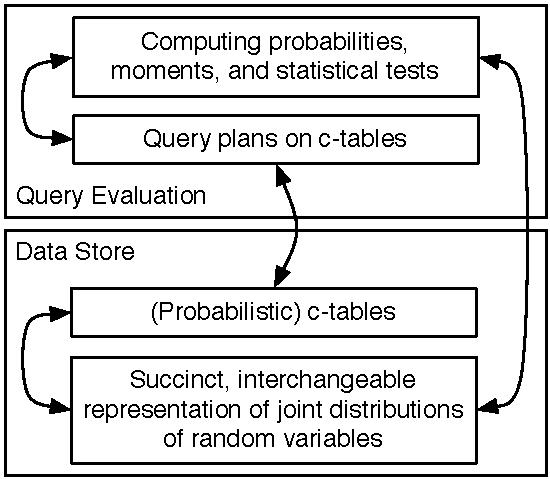
\includegraphics[width=2in]{graphics/arch.pdf}
\vspace*{-0.1in}
\caption{Pip Query Engine Architecture}
\label{fig:arch}
\end{center}
\vspace*{-0.35in}
\end{figure}

\subsection{Symbolic Representation}
PIP represents probabilistic data values symbolically via random variables defined in terms of parametrized probability distribution classes.  PIP supports several generic classes of probability distributions (e.g., Normal, Uniform, Exponential, Poisson), and may be extended with additional classes.  Variables are treated as opaque while they are manipulated by traditional relational operators.  The resulting symbolic representation is a c-table.  As the final stage of the query, special operators defined within PIP compute expectations and moments of the uncertain data, or sample the data to generate histograms.  

These expectation operators are invoked with an unbiased, lossless representation of the expression to be evaluated.  Because the variables have been treated as opaque, the expectation operator can obtain information about the distribution a variable corresponds to.  Developers can (but need not) provide supplemental information (e.g., functions defining the PDF and the CDF) about distributions they extend PIP with.  The operator can exploit this additional information to accelerate the sampling process, or potentially even sidestep it entirely.  For example, if a query asks for the probability that a variable will fall within specified bounds, the expectation operator can compute it with at most two evaluations of the variable's CDF.

Because the symbolic representation PIP uses is lossless, intermediate query results or views may be materialized.  Expectations of values in these views or subsequent queries based on them will not be biased by estimation errors introduced by materializing the view.  This is especially useful when a significant fraction of query processing time is devoted to managing deterministic data (eg, to obtain parameters for the model's variables).  Not only can this accelerate processing of commonly used subqueries, but it makes online sampling feasible; the sampler need not evaluate the entire query from scratch to generate additional samples.

\begin{example}\em
Consider the running example in the context of c-tables. The result of the relational algebra part of the
example query can be easily computed as
\[
\begin{tabular}{c|c|c}
R & Price & Condition \\
\hline
& $X_1$ & $X_2 \ge 7$ \\
\end{tabular}
\]
without looking at $p$.
This c-table compactly represents all data still relevant after the
application of the relational algebra part of the query, other than $p$,
which remains unchanged.
Sampling from R to compute
\begin{verbatim}
select expected_sum(Price) from R;
\end{verbatim}
is a much more focused effort.
First, we only have to consider the random variables relating to Joe;
but determining that random variable $X_2$ is relevant while $X_4$
is not requires
executing a query involving a join. We want to do this query first, before
we start sampling.

Second, assume that delivery times are
independent from sales volumes. Then we can approximate the
query result
by first sampling an $X_2$ value and only sampling an $X_1$ value if $X_2 \ge 7$.
Otherwise, we use $0$ as the $X_1$ value.
If $X_2 \ge 7$ is relatively rare (e.g., the average shipping times to NY are
very slow, with a low variance), this may reduce the amount of samples
for $X_1$ that are first computed and then discarded without seeing use
considerably.
If CDFs are available, we can of course do even better.
%
\end{example}

\subsection{Random Variables}

At the core of PIP's symbolic representation of uncertainty is the random variable, represented in PIP as a 4-tuple.  Each random variable consists of a unique identifier, a subscript (for multi-variate distributions), a distribution class, and a set of parameters for the distribution.  

For example, we write 
$$[X\Rightarrow Normal(\mu,\sigma^2)]$$
 to represent a normally distributed random variable $X$ with mean $\mu$ and standard deviation $\sigma^2$.  Multivariate distributions may be written in the form 
$$[X[n]\Rightarrow MVNormal(\mu, \sigma^2, N)]$$

Thus, when instantiating a random variable, users specify both a distribution for the variable to be sampled from, and a parameter set for that distribution.  As a single variable may appear simultaneously at multiple points within the database, the unique identifier is used to ensure that sampling processes generate consistent values for the variable within a given sample.  

Random variables are stored, either directly or as arithmetic formulas, in the tables of a database.  The equation datatype used for this purpose is simply a flattened parse tree of the formula.  Observe that while we limit our implementation to arithmetic operators, any non-recursive expression may be similarly represented; The equation datatype can potentially be used to encode any target expression accepted by PostgreSQL.  

Random variable equations can be combined freely with constant expressions, both in the target clause of a select statement, and in the where clause.  All targets including random variable equations are encoded as random variable equations themselves.  All where clauses including random variable equations are encoded as c-table conditions.  As this allows a variable to appear several times in a given context, the variable's identifier is used as part of the seed for the pseudorandom number generator used by the sampling processes.

C-table conditions allow PIP to represent per-tuple uncertainty.  Each tuple is tagged with a condition that must hold for the variable to be present in the table.  C-table conditions are expressed as a boolean equation of \textit{atoms}, arbitrary inequalities of random variables.  The independent probability, or \textit{confidence} of the tuple is the probability of the condition being satisfied.  

Given  tables  in which  all  conditions  are  conjunctions of  atomic conditions and  the query does not employ  duplicate elimination, then all conditions  in the output  table are conjunctions.  Thus  it makes sense to particularly optimise this scenario \cite{AJKO2008}. In the case of positive relational algebra  with the duplicate elimination  operator (i.e., we trade  duplicate   elimination  against  difference),   we  can  still efficiently  maintain  the  conditions  in  DNF,  i.e.,  as  a  simple disjunction of conjunctions of atomic conditions.

Without loss of generality, the model can be limited to conditions that are conjunctions of constraint  atoms.  Generality  is maintained by  using bag  semantics to encode disjunctions. This  restriction   provides   several  benefits. First, constraint  validation is  simplified;  A pairwise  comparison of  all atoms in the clause is  sufficient to catch the inconsistencies listed above.   As an additional  benefit, if  all atoms  of a  clause define convex and  contiguous regions in the space $\vec{x},\vec{y}$, these same properties are also shared by their intersection.

\subsection{Condition Inconsistency}
Conditions can become \textit{inconsistent} by combining contradictory conditions using conjunction, which may happen in the implementations of the operators selection, product, and difference.  If such tuples are discovered, they may be freely removed from the c-table.  

A condition is consistent if there is a variable assignment that makes the condition true. For general boolean formulas, deciding consistency is computationally hard. But we do not need to decide it during the evaluation of relational algebra operations.  Rather, we exploit straightforward cases of inconsistency to clean-up c-tables and reduce their sizes. We rely on the later Monte Carlo simulation phase to enforce the remaining inconsistencies.
%
\begin{enumerate}
\item The consistency of conditions not involving variable values is always immediately apparent.
\item Conditions $X_i = c_1 \land X_i = c_2$ with constants $c_1 \neq c_2$ are always inconsistent.
\item Equality conditions over continuous variables $Y_j = (\cdot)$, with the exception of the identity $Y_j = Y_j$, are not inconsistent but can be treated as such (the probability mass will always be zero).  Similarly, conditions $Y_j \neq (\cdot)$, with the exception of $Y_j \neq Y_j$, can be treated as true and removed or ignored.
\item Other forms of inconsistency can also be detected where it is efficient to do so.
\end{enumerate}

With  respect to discrete variables, inconsistency detection may be further simplified.  Rather than using abstract representations, every row containing discrete variables may be exploded into one row for every possible valuation.  Condition atoms matching each variable to its valuation are used to ensure mutual exclusion of each row.  Thus, discrete variable columns may be treated as constants for the purpose of consistency checks.  As shown in \cite{AJKO2008}, deterministic database query optimizers do a satisfactory job of ensuring that constraints over discrete variables are filtered as soon as possible.

%\vspace*{0.05in}
\begin{figure}
\begin{algorithm} Checking the consistency of a condition
\label{alg:consistCheck}
\footnotesize
\begin{enumerate}
\item $consistencyCheck($ConditionSet $C)$
\item \hspace*{0.1in} foreach \textit{Discrete} condition $[X = c_1] \in C$
\item \hspace*{0.2in} if $\exists [X = c_2] \in C$ s.t. $c_1 \neq c_2$, return \textbf{Inconsistent.}
\item \hspace*{0.1in} foreach \textit{Continuous} variable group $K$ (See Section \ref{subsec:samplingTechs})
\item \hspace*{0.2in} initialize map $S_0$ s.t. $S_0[X] = [-\infty,\infty]\ \forall X \in K$
\item \hspace*{0.2in} while $S_{t} \neq S_{t-1}$ (incrementing $t>0$ each iteration)
\item \hspace*{0.3in} let $S_{t} = S_{t-1}$
\item \hspace*{0.3in} foreach equation $E \in K$
\item \hspace*{0.4in} if $\exists$ no more than one $X\in E$ s.t. $S_{t-1}[x] = [-\infty,\infty]$
\item \hspace*{0.5in} foreach $X$, $S_{t}[X] = S_{t-1} \cap tighten_N(X,E,S_{t})$\\ \hspace*{0.7in} (Where $N = $ the degree of E)
\item \hspace*{0.5in} if $tighten_N$ has not been defined, skip $E$.
\item \hspace*{0.3in} if $\exists X$ s.t. $S_{t}[X] = \emptyset$, return \textbf{Inconsistent.}
\item \hspace*{0.1in} if no Eqns were skipped return \textbf{Consistent.} else return \textit{Consistent.}
\end{enumerate}
\begin{enumerate}
\item $tighten_1($Variable $X,$ Equation $E,$ IntervalMap $S)$
\item \hspace*{0.1in} Express E in normal form $aX + bY + cZ + \ldots > 0$
\item \hspace*{0.2in} if $a > 0$, return $[-\max_{S[Y,Z,\ldots]}(bY+cZ+\ldots)/a, \infty]$
\item \hspace*{0.2in} if $a < 0$, return $[-\infty, -\max_{S[Y,Z,\ldots]}(bY+cZ+\ldots)/a]$
\end{enumerate}
\end{algorithm}
{\footnotesize Strong consistency guarantees returned by this algorithm are marked in \textbf{bold}, while weak ones are marked in \textit{italics}.}
\vspace*{-0.2in}
\end{figure}

This sampling algorithm is presented in Algorithm \ref{alg:consistCheck}.  Due to space constraints only $tighten_1$ is presented in this paper, but all polynomial equations may be handled using a similar, albeit more complex enumeration of coefficients\footnote{PIP limits itself to 2nd degree polynomials}.  We have decided to limit PIP to simple algebraic operators in the current implementation, thus all variable expressions are polynomial.  As this process is optional, more complex equations need not be handled by it.

\subsection{Distributions}
As variables are defined in terms of parametrized distribution classes, PIP's infrastructure is agnostic to the implementation of the underlying distributions.  When defining a distribution, programmers need only include a mechanism for sampling from that distribution; much like \cite{MCDB}'s VG Functions.  However, PIP is not limited to simple sampling functionality.  If it is possible to efficiently compute or estimate the distribution's probability density function ($PDF$), cumulative distribution function ($CDF$), and/or inverse cumulative distribution function ($CDF^{-1}$), these may be included to improve PIP's efficiency.  

Distribution specific values like the $PDF$, $CDF$ and inverse $CDF$ are used to demonstrate what can be achieved with PIP's framework.  Further distribution-specific values like weighted-sampling, mean, entropy, and the higher moments can be used by more advanced statistical methods to achieve even better performance.  The process of defining a variable distribution is described further in Section \ref{sec:implementation}.  

Though PIP abstracts the details of a variable's distribution from query evaluation, it distinguishes between discrete and continuous distributions.  As described in Section \ref{sec:background}, existing research into c-tables has demonstrated efficient ways of querying variables sampled from discrete distributions.  PIP employs similar techniques when it is possible to do so.

